\chapter{Supporting Material for Chapter 2, Method}
\label{cha:app2}
\section{Codebase and data}
The modelling and data analysed for this thesis were done in the R programming language. The complete codebase created for this thesis and the required raw data to execute the code are available via GitHub.\\
%%%%LINK !Github!!!!!!
Some basic instructions on running the code are provided in the ReadMe and comment sections. For further questions please contact via email at: juan.bettinelli@tum.de or bettinelli.jb@googlemail.com



\section{Figures App. ch.2}
\begin{figure}[htbp]
 \centering
 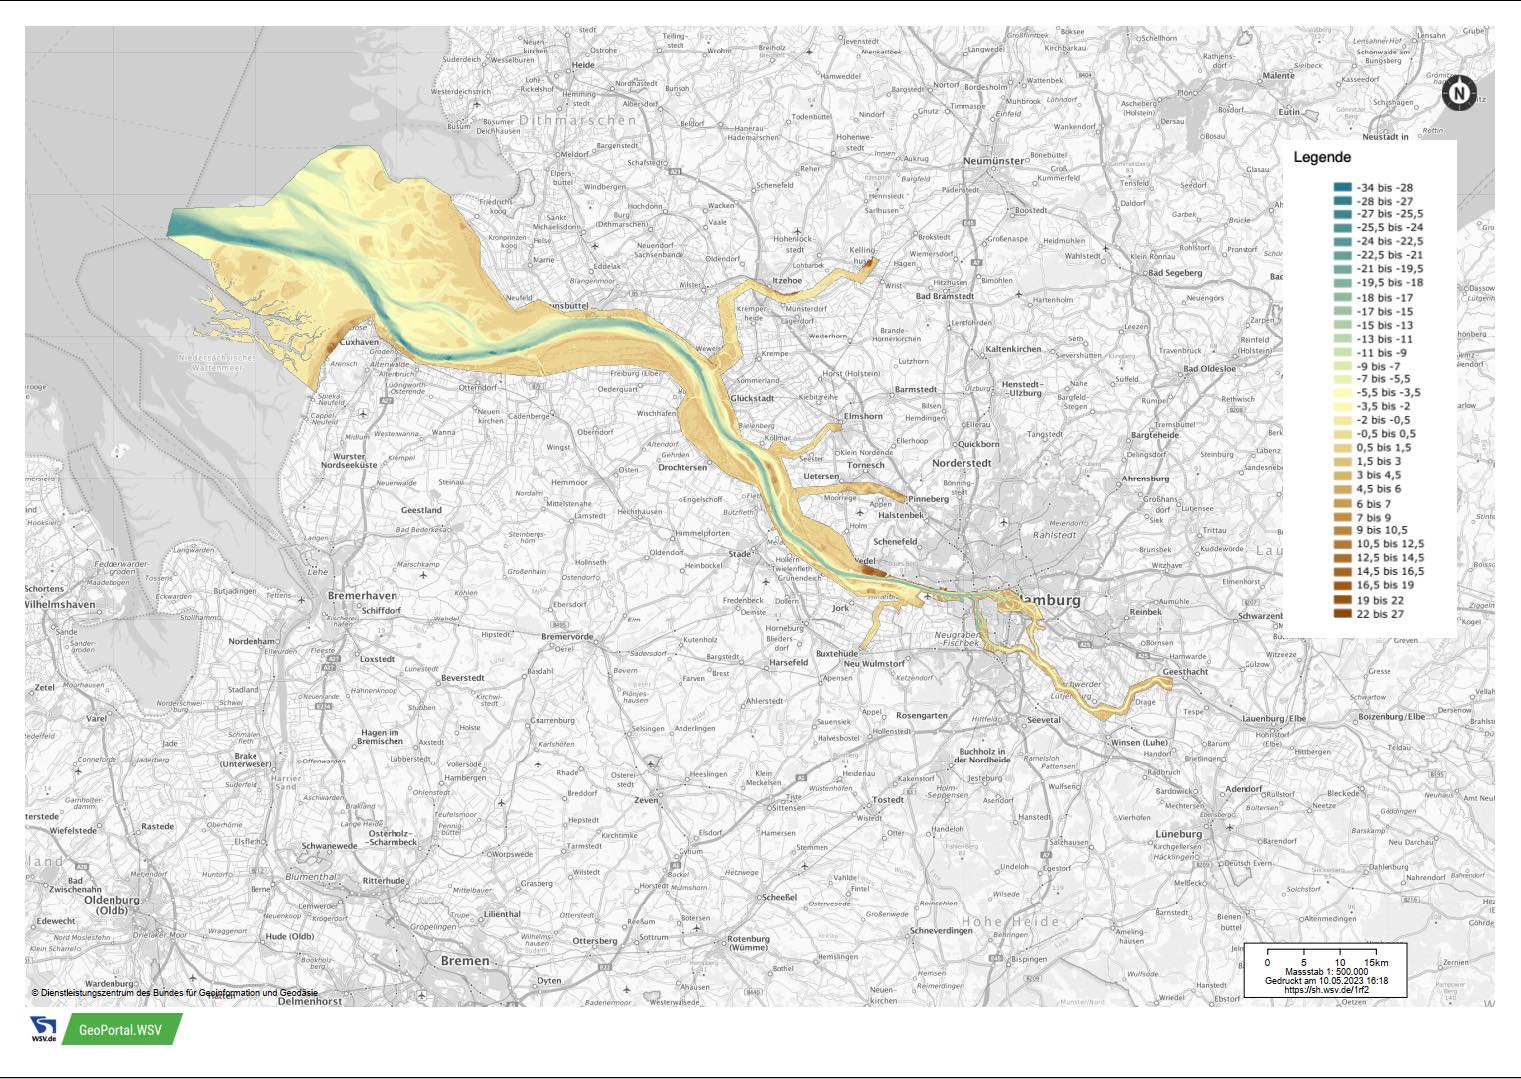
\includegraphics[width=1\textwidth]{figures/Appendix/Map/TopographieElbeGesamt.jpg}
 \caption[Topographic map of Elbe]{Topographic map of the estuary of Elbe. From the Hamburg region to the Waddensea. Scale is in dm, 0 dm is at mean sea level. \cite{ZDMGDWS.2016}}
 \label{TopographyElbeTotal}
\end{figure}